\documentclass[10pt]{article}

\usepackage[T1]{fontenc}
\usepackage{geometry}
\usepackage{amsmath, amssymb, amsthm}
\usepackage{graphicx}
\usepackage{float}
\usepackage{multirow}
\usepackage{bm}
\usepackage{hyperref}

\geometry{a4paper, margin=1in}

\renewcommand{\labelenumi}{(\alph{enumi})}
\renewcommand{\vec}{\bm}

\DeclareMathOperator{\rank}{rank}
\DeclareMathOperator{\col}{col}

\newcommand{\C}{\mathbb{C}}
\newcommand{\R}{\mathbb{R}}
\newcommand{\Q}{\mathbb{Q}}
\newcommand{\Z}{\mathbb{Z}}
\newcommand{\N}{\mathbb{N}}

\setlength{\parindent}{0em}

\title{Assignment I}
\author{Satvik Saha}
\date{}

\begin{document}
    \noindent\textbf{IISER Kolkata} \hfill \textbf{Assignment II}
    \vspace{3pt}
    \hrule
    \vspace{3pt}
    \begin{center}
    \LARGE{\textbf{MA4206: Linear Models}}
    \end{center}
    \vspace{3pt}
    \hrule
    \vspace{3pt}
    Satvik Saha, \texttt{19MS154} \hfill \today
    \vspace{20pt}

    \setlength{\parskip}{1em}


    \section{Introduction}

    There are 33 countries with data on umemployment rates, GDP per capita, and total
    investment as a percentage of GDP, denoted UNMP ($y$), GDP ($x_1$), INV ($x_2$)
    respectively.


    These are fitted against the linear model \[
        y_i = \beta_0 + \beta_1 x_{i1} + \beta_2 x_{i2} + \epsilon_i. \tag{$\star$}
    \]

    The fitted parameters are as follows, with an adjusted $R^2$ value of 0.477.

    \begin{table}[H]
        \centering
        \caption{Fitted parameters from the linear model $(\star)$.}
        \vspace{1em}
        \label{tab:parameters}
        \begin{tabular}{rccc}
            \hline
                & Variable & Value & Standard error \\\hline
            Intercept & $\beta_0$ & $2.639 \times 10^1$ &  $0.347 \times 10^1$ \\
            GDP & $\beta_1$ & $-7.926 \times 10^{-5}$ & $3.204 \times 10^{-5}$ \\
            INV & $\beta_2$ & $-7.051 \times 10^{-1}$ & $1.598 \times 10^{-1}$ \\\hline
        \end{tabular}
    \end{table}

    We further plot fitted values of UNMP vs observed values of UNMP.

    \begin{figure}[H]
    \begin{center}
        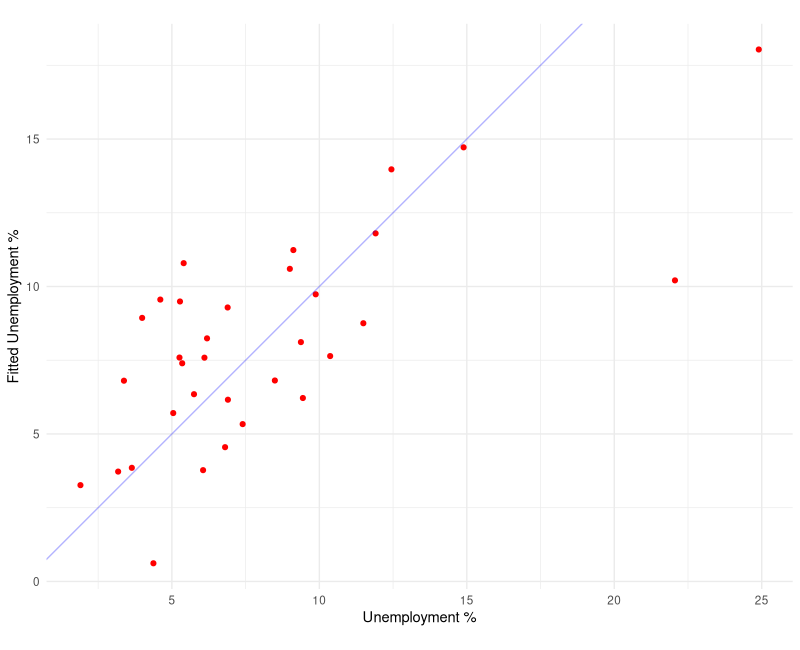
\includegraphics[width=0.8\textwidth]{scatter.png}
    \end{center}
    \caption{UNMP values, fitted vs actual. The blue line marks $x = y$.}
    \label{fig:scatter}
    \end{figure}

    From the above plot, we see that the model performs especially badly on the two
    points on the extreme right, which represent the countries Greece and Spain.
    Elsewhere, the model seems to explain the general trend of observed values,
    albeit poorly. Thus, the goodness of fit is poor.

    Plotting the residuals vs fitted UNMP values further highlights that Greece and
    Spain are outliers (with the highest residual values). Although $\hat{\epsilon}$
    and $\hat{y}$ are uncorrelated, we calculate a Spearman correlation of -0.24.

    \begin{figure}[H]
    \begin{center}
        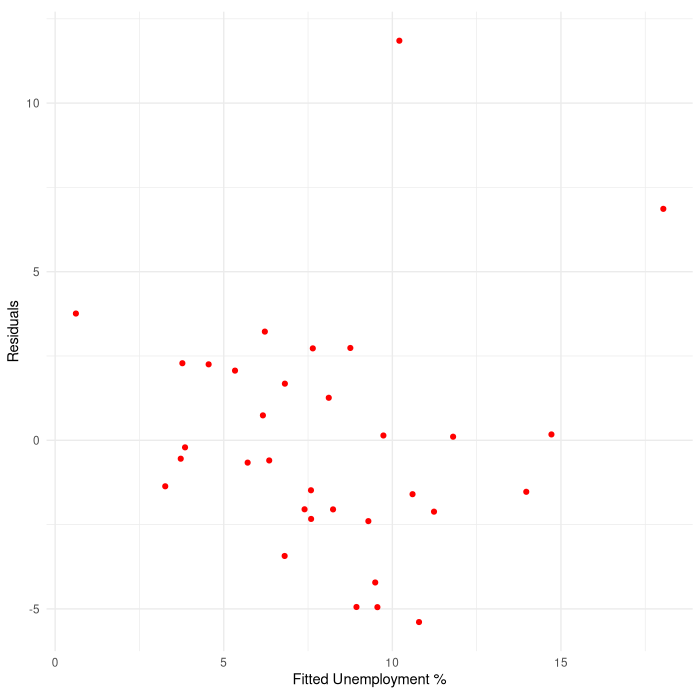
\includegraphics[width=0.8\textwidth]{residuals.png}
    \end{center}
    \caption{Residuals vs fitted values of UNMP.}
    \label{fig:residuals}
    \end{figure}


    \section{Prediction intervals}

    The 95\% prediction intervals for the model have been calculated and displayed
    below.

    \begin{figure}[H]
    \begin{center}
        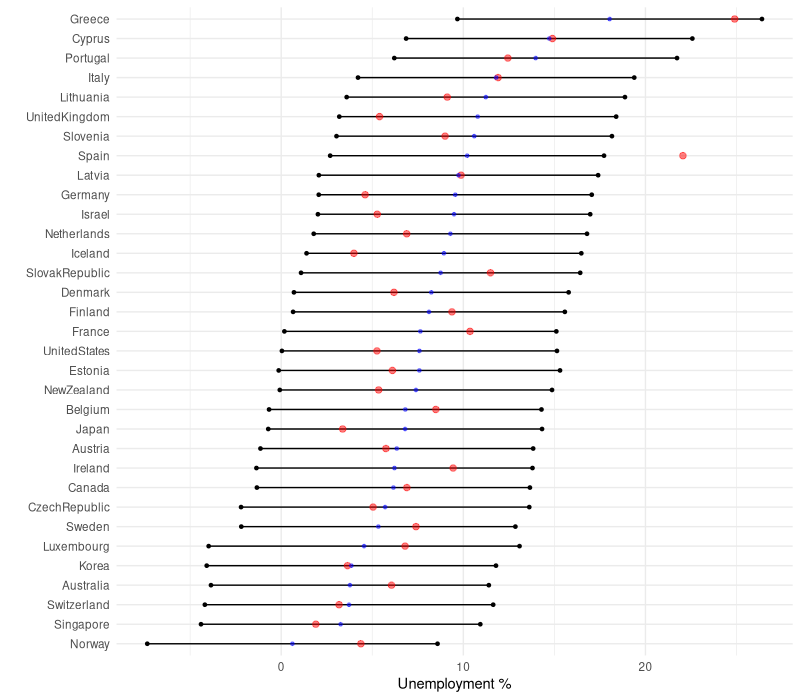
\includegraphics[width=0.8\textwidth]{predicted_intervals.png}
    \end{center}
    \caption{Prediction intervals for UNMP. The blue points mark the fitted values,
    while the red points mark the observed values.}
    \label{fig:prediction}
    \end{figure}



    \section{Leave One Out Cross Validation}

    We perform Leave One Out Cross Validation (LOOCV) by fitting the model against
    the data with the $i$-th entry removed, for each of the 33 rows indexed by $i$.
    The tuples of fitted parameters $(\beta_0^{(i)}, \beta_1^{(i)}, \beta_2^{(i)})$
    have been plotted in space, with the points labelled by the $i$-th country.

    \begin{table}[H]
        \centering
        \caption{Fitted parameters from the linear model $(\star)$ with the $i$-th
        entry removed.}
        \vspace{1em}
        \label{tab:parameters_loocv}
        \begin{tabular}{rlrrr}
          \hline
         $i$ & Country & $\beta_0^{(i)}$ & $\beta_1^{(i)}$ & $\beta_2^{(i)}$ \\
          \hline
              1 & Australia & 26.826 & -0.0000805 & -0.727 \\
              2 & Austria & 26.355 & -0.0000792 & -0.703 \\
              3 & Belgium & 26.457 & -0.0000791 & -0.711 \\
              4 & Canada & 26.441 & -0.0000793 & -0.708 \\
              5 & Cyprus & 26.319 & -0.0000791 & -0.702 \\
              6 & CzechRepublic & 26.257 & -0.0000810 & -0.694 \\
              7 & Denmark & 26.558 & -0.0000767 & -0.715 \\
              8 & Estonia & 26.282 & -0.0000827 & -0.691 \\
              9 & Finland & 26.338 & -0.0000795 & -0.704 \\
              10 & France & 26.394 & -0.0000785 & -0.711 \\
              11 & Germany & 26.985 & -0.0000779 & -0.728 \\
              12 & Greece & 21.339 & -0.0000712 & -0.498 \\
              13 & Iceland & 26.955 & -0.0000739 & -0.734 \\
              14 & Ireland & 26.431 & -0.0000849 & -0.701 \\
              15 & Israel & 26.809 & -0.0000802 & -0.717 \\
              16 & Italy & 26.366 & -0.0000792 & -0.704 \\
              17 & Japan & 26.184 & -0.0000815 & -0.686 \\
              18 & Korea & 26.328 & -0.0000797 & -0.701 \\
              19 & Latvia & 26.382 & -0.0000789 & -0.706 \\
              20 & Lithuania & 26.688 & -0.0000837 & -0.708 \\
              21 & Luxembourg & 26.345 & -0.0000965 & -0.676 \\
              22 & Netherlands & 26.664 & -0.0000780 & -0.717 \\
              23 & NewZealand & 26.355 & -0.0000799 & -0.699 \\
              24 & Norway & 27.688 & -0.0000892 & -0.753 \\
              25 & Portugal & 26.902 & -0.0000813 & -0.723 \\
              26 & Singapore & 26.093 & -0.0000783 & -0.691 \\
              27 & SlovakRepublic & 26.398 & -0.0000732 & -0.721 \\
              28 & Slovenia & 26.582 & -0.0000817 & -0.707 \\
              29 & Spain & 25.068 & -0.0000666 & -0.685 \\
              30 & Sweden & 26.590 & -0.0000806 & -0.715 \\
              31 & Switzerland & 26.330 & -0.0000772 & -0.705 \\
              32 & UnitedKingdom & 27.505 & -0.0000755 & -0.756 \\
              33 & UnitedStates & 26.514 & -0.0000759 & -0.714 \\
           \hline
        \end{tabular}
    \end{table}

    If the fitted parameters for some $i$  deviate significantly from the rest, we
    hypothesize that the corresponding country heavily influences our model. Indeed,
    the countries Greece and Spain deviate the most.

    This degree of outlyingness can be loosely quantified by the Mahalanobis depth,
    also indicated in a figure below.

    \begin{figure}[H]
    \begin{center}
        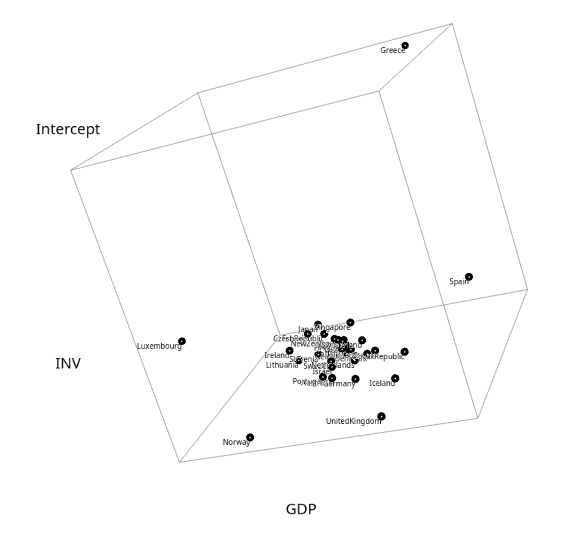
\includegraphics[width=0.9\textwidth]{loocv.png}
    \end{center}
    \caption{Fitted parameter values obtained from the linear model upon removing the
    entry with the labelled country.}
    \label{fig:loocv}
    \end{figure}

    \begin{figure}[H]
    \begin{center}
        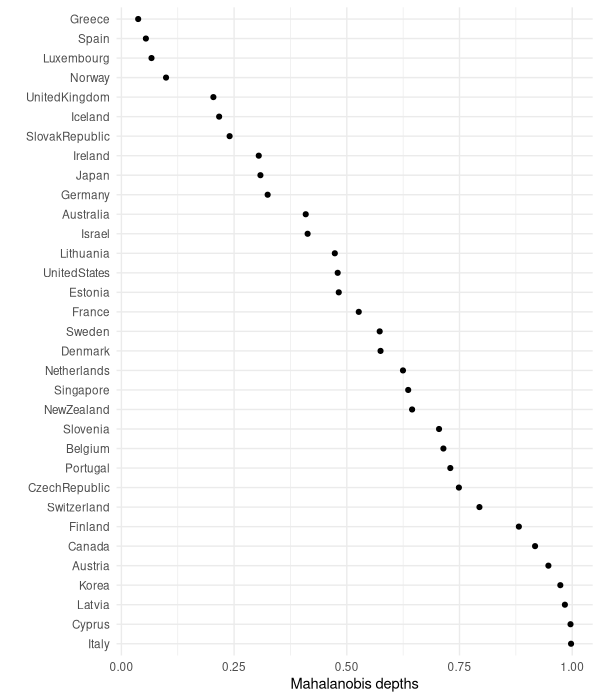
\includegraphics[width=0.7\textwidth]{mahalanobis_depths}
    \end{center}
    \caption{Mahalanobis depths of the data points in Figure \ref{fig:loocv}.}
    \label{fig:depths}
    \end{figure}


    \section{Removing outliers}

    We removed the rows corresponding to the countries Greece and Spain, and perform
    the same procedures as before. Our new parameter estimates are given below, with
    an adjusted $R^2$ of 0.415.

    \begin{table}[H]
        \centering
        \caption{Fitted parameters from the linear model $(\star)$.}
        \vspace{1em}
        \label{tab:parameters_reduced}
        \begin{tabular}{rccc}
            \hline
                & Variable & Value & Standard error \\\hline
            Intercept & $\beta_0^*$ & $1.923 \times 10^1$ &  $0.272 \times 10^1$ \\
            GDP & $\beta_1^*$ & $-5.655 \times 10^{-5}$ & $2.124 \times 10^{-5}$ \\
            INV & $\beta_2^*$ & $-4.481 \times 10^{-1}$ & $-3.717 \times 10^{-1}$ \\\hline
        \end{tabular}
    \end{table}

    The fitted vs observed plot now exhibits a much more reasonable trend.

    \begin{figure}[H]
    \begin{center}
        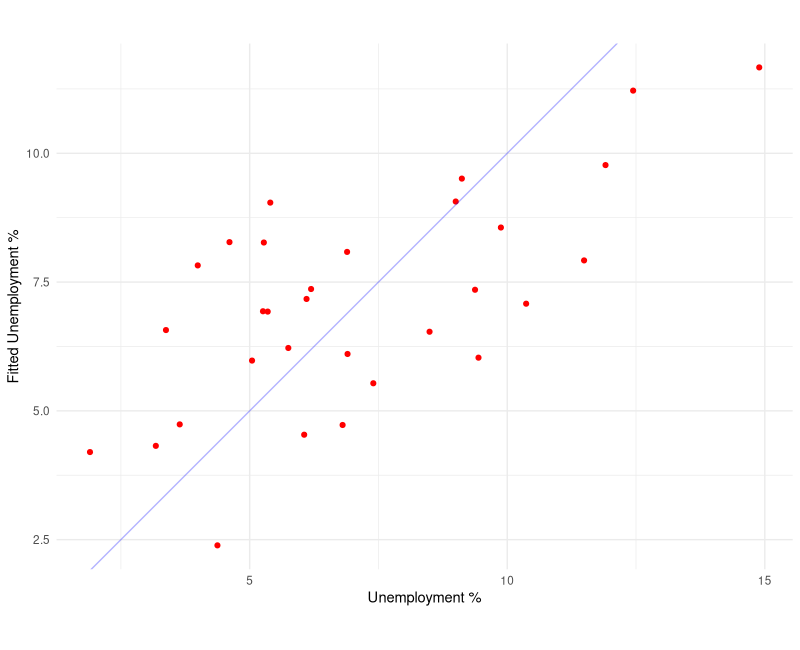
\includegraphics[width=0.7\textwidth]{scatter_reduced.png}
    \end{center}
    \caption{UNMP values, newly fitted vs actual. The blue line marks $x = y$.}
    \label{fig:scatter_reduced}
    \end{figure}

    The residuals now exhibit a Spearman correlation of -0.04 with the newly fitted
    UNMP values.

    \begin{figure}[H]
    \begin{center}
        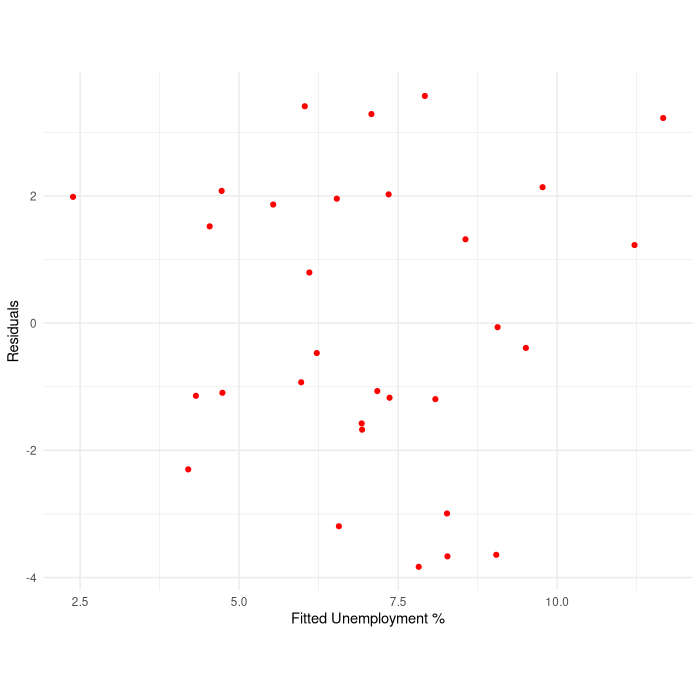
\includegraphics[width=0.7\textwidth]{residuals_reduced.png}
    \end{center}
    \caption{New residuals vs newly fitted values of UNMP.}
    \label{fig:residuals_reduced}
    \end{figure}

    \begin{figure}[H]
    \begin{center}
        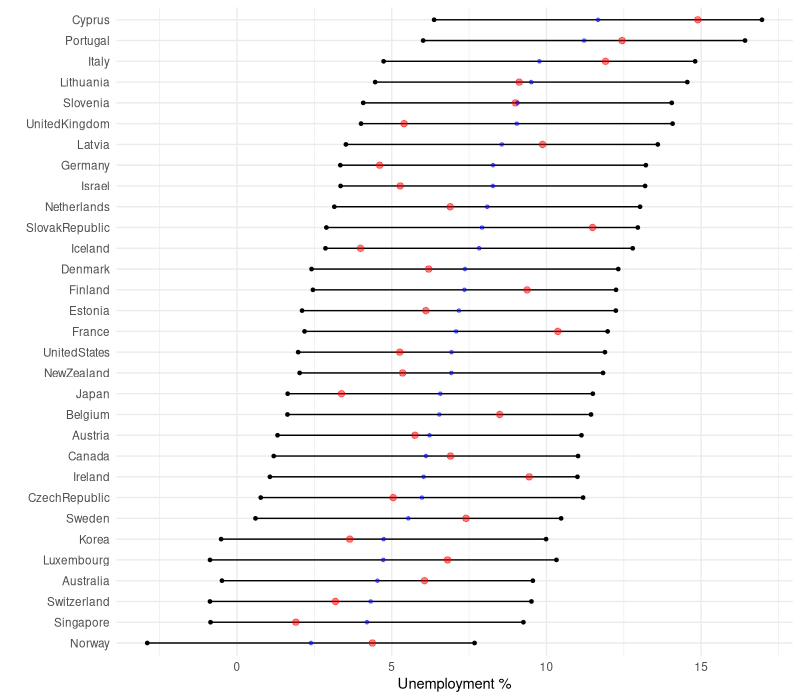
\includegraphics[width=0.8\textwidth]{predicted_intervals_reduced.png}
    \end{center}
    \caption{Prediction intervals for UNMP. The blue points mark the fitted values,
    while the red points mark the observed values.}
    \label{fig:prediction_reduced}
    \end{figure}

    \begin{figure}[H]
    \begin{center}
        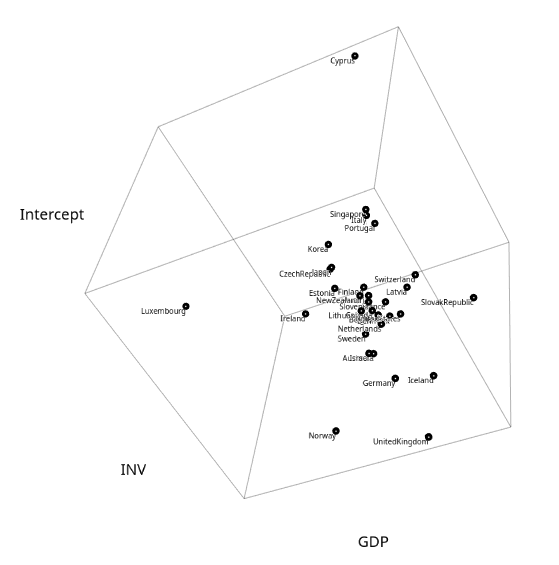
\includegraphics[width=0.9\textwidth]{loocv_reduced.png}
    \end{center}
    \caption{New fitted parameter values obtained from the linear model upon removing
    the entry with the labelled country.}
    \label{fig:loocv_reduced}
    \end{figure}


    \section{Discussion}

    We have justified the removal of the countries Greece and Spain on the basis of
    their position in the fitted vs observed and residual vs fitted plots, as well as
    their outlyingness in the LOOCV fitted parameter scatter plot. With this, the
    remaining countries fit reasonably well in the model; the next candidate
    countries for removal would be Cyprus and Luxembourg.

    These two countries exhibit an unemployment rate that is significantly higher
    than predicted. Thus, it indicates that their economics scenarios are very
    different from those of the remaining countries, which can be somewhat accurately
    modelled using only two variables.

    \begin{figure}[H]
    \begin{center}
        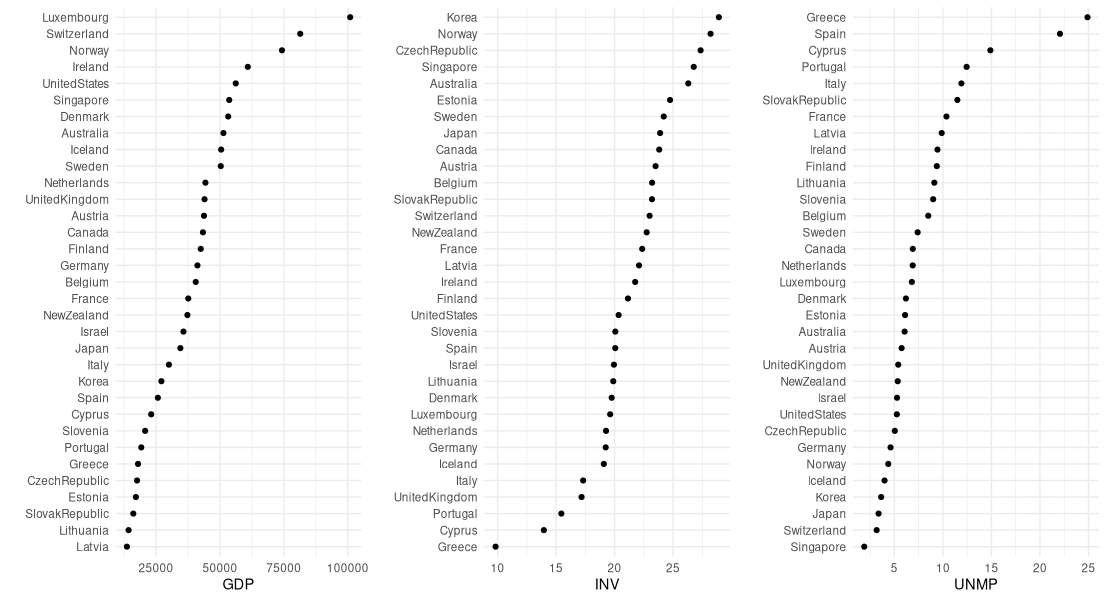
\includegraphics[width=\textwidth]{gdp_inv_unmp.png}
    \end{center}
    \caption{Sorted values of GDP, INV, and UNMP.}
    \label{fig:gdp_inv_unmp}
    \end{figure}

    We note that Greece has the lowest total investment rate by far, followed by
    Cyprus and Portugal, which may help explain Greece's status as an outlier.
    Additionally, Luxembourg has the highest GDP by far, followed by Switzerland and
    Norway.



\end{document}
